%\chapter{Algumas Demonstra{\c c}\~oes}
%\chapter{Estimação da posição e orientação}
\chapter{Estimação \textit{online} da \textit{pose}}  \label{chap:pose_est}
\section{ViSP - Visual Servoing Platform}

Para a implementação do modo de controle por Servo Visão, foi utilizada a biblioteca ViSP. A ViSP contém um módulo de visão computacional que permite computar a \textit{pose} de um objeto a ser reconhecido por meio de um padrão pre-determindado. São utilizados algoritmos robustos e fornecidos mecanismos para calibração da câmera. Esse módulo em alguns casos utiliza a biblioteca OpenCV, de modo a facilitar sua aplicação em problemas de robótica. 
%funciona como um envoltório para a
\section{Rastreamento Baseada em Modelo}
O ViSP propoe um rastreador baseado em modelo 3D que permite simultaneamente rastrear um objeto utilizando conhecimento de seu modelo CAD e fornecer a sua posição e  orientação, no sistema de coordenadas da câmera.

O rastreamento é dividido em duas etapas. A primeira consiste em rastrear as características do objeto. A segunda etapa consiste em determinar a \textit{pose} da câmera para fazer a correspondência das características rastreadas com a projeção do modelo 3D.

Dependendo das características visuais, três rastreadores estão disponíveis.
\begin{itemize}
\item Rastreador que considera bordas móveis. Esse rastreador é apropriado para objetos não texturizados.
\item Rastreador pelo algoritmo Kanade–Lucas–Tomasi \citep{tomasi1991detection}, conhecido como KLT. Esse modo é projetado para objetos texturizados cujas boradas não são bem visíveis.
\item Versão híbrida que considera bordas móveis e pontos chave KLT. 
\end{itemize}

\begin{figure}[!ht]
\centering
  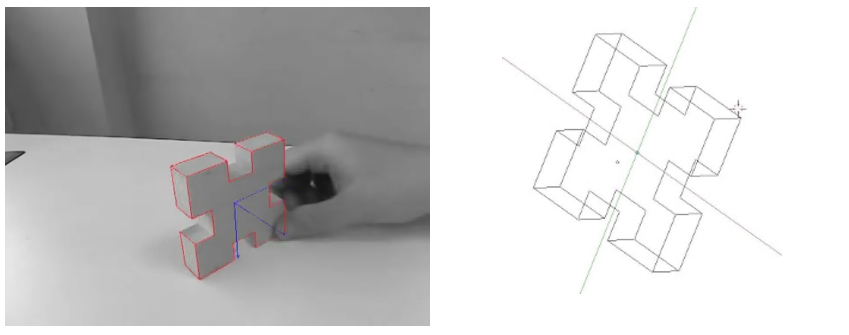
\includegraphics[width=\linewidth]{./img/visp.png}
  \caption{Rastreamento baseado em modelo}
  \label{fig:cenpes_doris}
\end{figure}%

\section{Perspective-n-Point}
As seguintes abordagens ao problema PnP estão disponíveis
\begin{itemize}
\item Abordagem Linear Lagrange. É realizado um teste para verificar aplicação da versão planar ou não-planar do algoritmo. 

\item Abordagem Linear Dementhon \citep{dementhon1995model, oberkampf1996iterative}  É realizado um teste para verificar aplicação da versão planar ou não-planar do algoritmo. 
	
\item Abordagem Lowe baseada em um esquema de minimização não linear de Levenberg Marquartd. Precisa de inicialização por meio de Lagrange ou Dementhon.

\item  Abordagem de Lowe: Baseia-se em uma minimização não linear, inicializada pela aboradagem de Lagrange.
\end{itemize}

\section{Pacote de ROS visp\_auto\_tracker}
O pacote de ROS chamado \verb|visp_auto_tracker| consiste em um rastreador de objetos baseado em padrões. Ele funciona como um envoltório de ROS para rastreadores baseados em modelo fornecidos pela biblioteca de servo visão ViSP. O objeto a ser rastreado deve possuir um \textit{QRCode} ou um padrão \textit{Flash}. Baseado nesse padrão, o objeto é detectado automaticamente, permitindo a inicialização de rastreadores baseados em modelo. Quando o rastreamento se perde, uma nova detecção é feita e os rastreador é re-inicializado.

O algoritmo utilizado para a solução do problema Perspective-n-Point é a abordagem descrita em \citep{dementhon1995model,oberkampf1996iterative}, que permite computar a posição e orientação rápido o suficiente para permitir rastreio \textit{online} utilizando uma câmera.

\begin{figure}[!ht]
\centering
  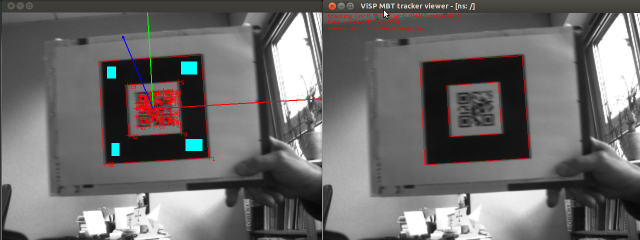
\includegraphics[width=\linewidth]{./img/tracker_viewer-small.png}
  \caption{Rastreamento de um QRCode}
  \label{fig:cenpes_doris}
\end{figure}%


